\chapter{基于SBAS-InSAR技术的地表形变检测}

\section{研究区域}

研究区域为卡尔斯巴德未坍塌的卤水井。如图\ref{fig:studyarea}中方框所圈的内容所示。
\begin{figure}[htb]
    \centering
    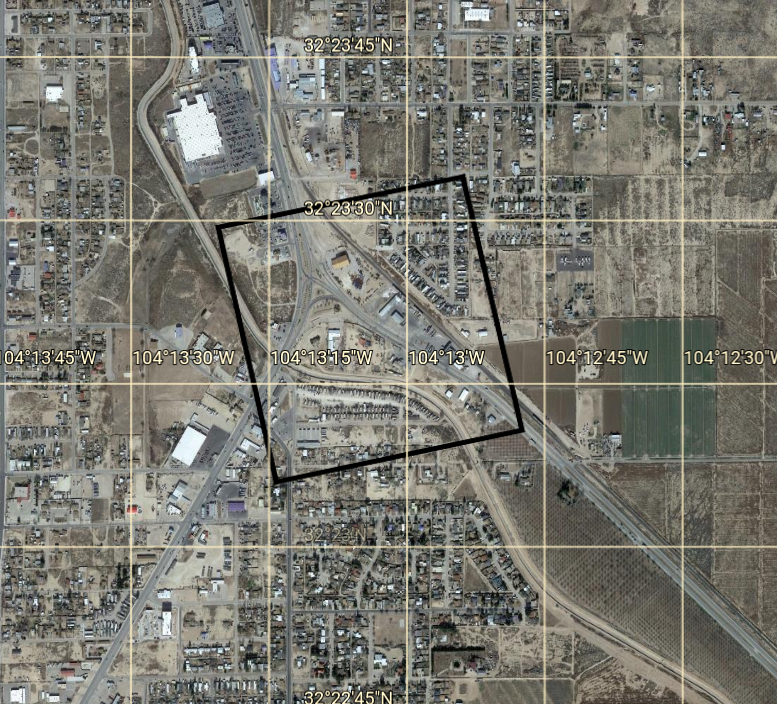
\includegraphics[width=0.8\textwidth]{studyarea.png}
    \caption{研究区域示意图}
    \label{fig:studyarea}
\end{figure}

\section{数据源}

本研究使用的数据为ALOS PALSAR的数据。
ALOS是日本与2006年发射的卫星,PALSAR为该卫星上搭载的L波段的合成孔径雷达。
数据的基本参数见表\ref{tab:palsar}。
\begin{table}[htb]
    \centering\small
    \caption{数据基本参数}
    \label{tab:palsar}
    \begin{tabular}{@{}cc@{}}
    \toprule
    参数           & 值                                \\ 
    \midrule
    雷达           & ALOS PALSAR                      \\
    中心频率         & 1270 MHz(L波段)                    \\
    range方向采样数   & 94                               \\
    azimuth方向采样数 & 252                              \\
    heading      & $-10.13^{\circ}$至$-10.18^{\circ}$ \\
    入射角          & $38.73^{\circ}$左右  \\
    \bottomrule
    \end{tabular}
\end{table}
监测时间从2006年12月到2011年2月共计15幅影像,详情参见表\ref{tab:timeseries}。
\begin{table}[htb]
    \centering\small
    \caption{数据时间序列}
    \label{tab:timeseries}
    \begin{tabular}{@{}cccc@{}}
    \toprule
    序号 & 成像时间 & 序号 & 成像时间\\ 
    \midrule
    1 & 2006.12.20 & 9 & 2010.05.15 \\
    2 & 2007.06.22 & 10 & 2010.06.30 \\
    3 & 2007.12.23 & 11 & 2010.08.15 \\
    4 & 2008.05.09 & 12 & 2010.09.30 \\
    5 & 2008.06.24 & 13 & 2010.11.15 \\
    6 & 2008.12.25 & 14 & 2010.12.31 \\
    7 & 2009.12.28 & 15 & 2011.02.15 \\
    8 & 2010.05.30 & & \\
    \bottomrule
    \end{tabular}
\end{table}
\section{数据处理}

本研究首先使用gamma软件进行干涉对的选择,选取2009年12月28日的影像为主影像,
结果如图\ref{fig:bprep}所示。
\begin{figure}[htb]
    \centering
    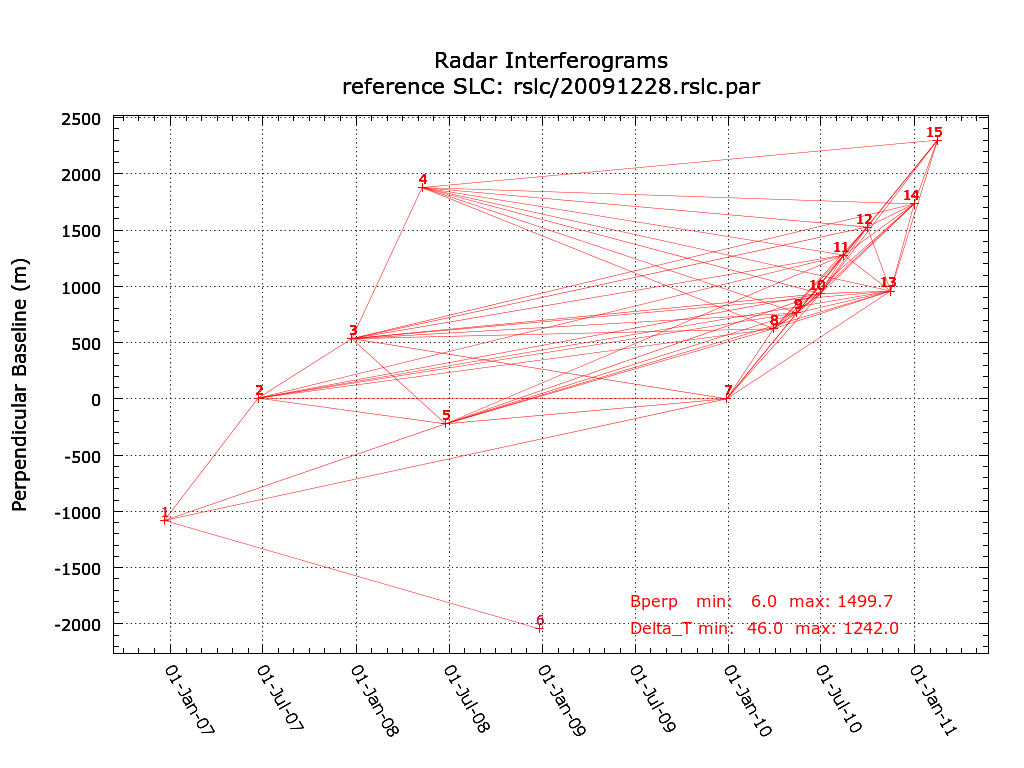
\includegraphics[width=0.8\textwidth]{bperp.png}
    \caption{时空基线连接图}
    \label{fig:bprep}
\end{figure}
然后使用StamPS软件进行SBAS技术数据处理。
处理所得平均速度如图\ref{fig:sbasv},相对的形变如图\ref{fig:sbasu}所示。
\begin{figure}[htb]
    \centering
    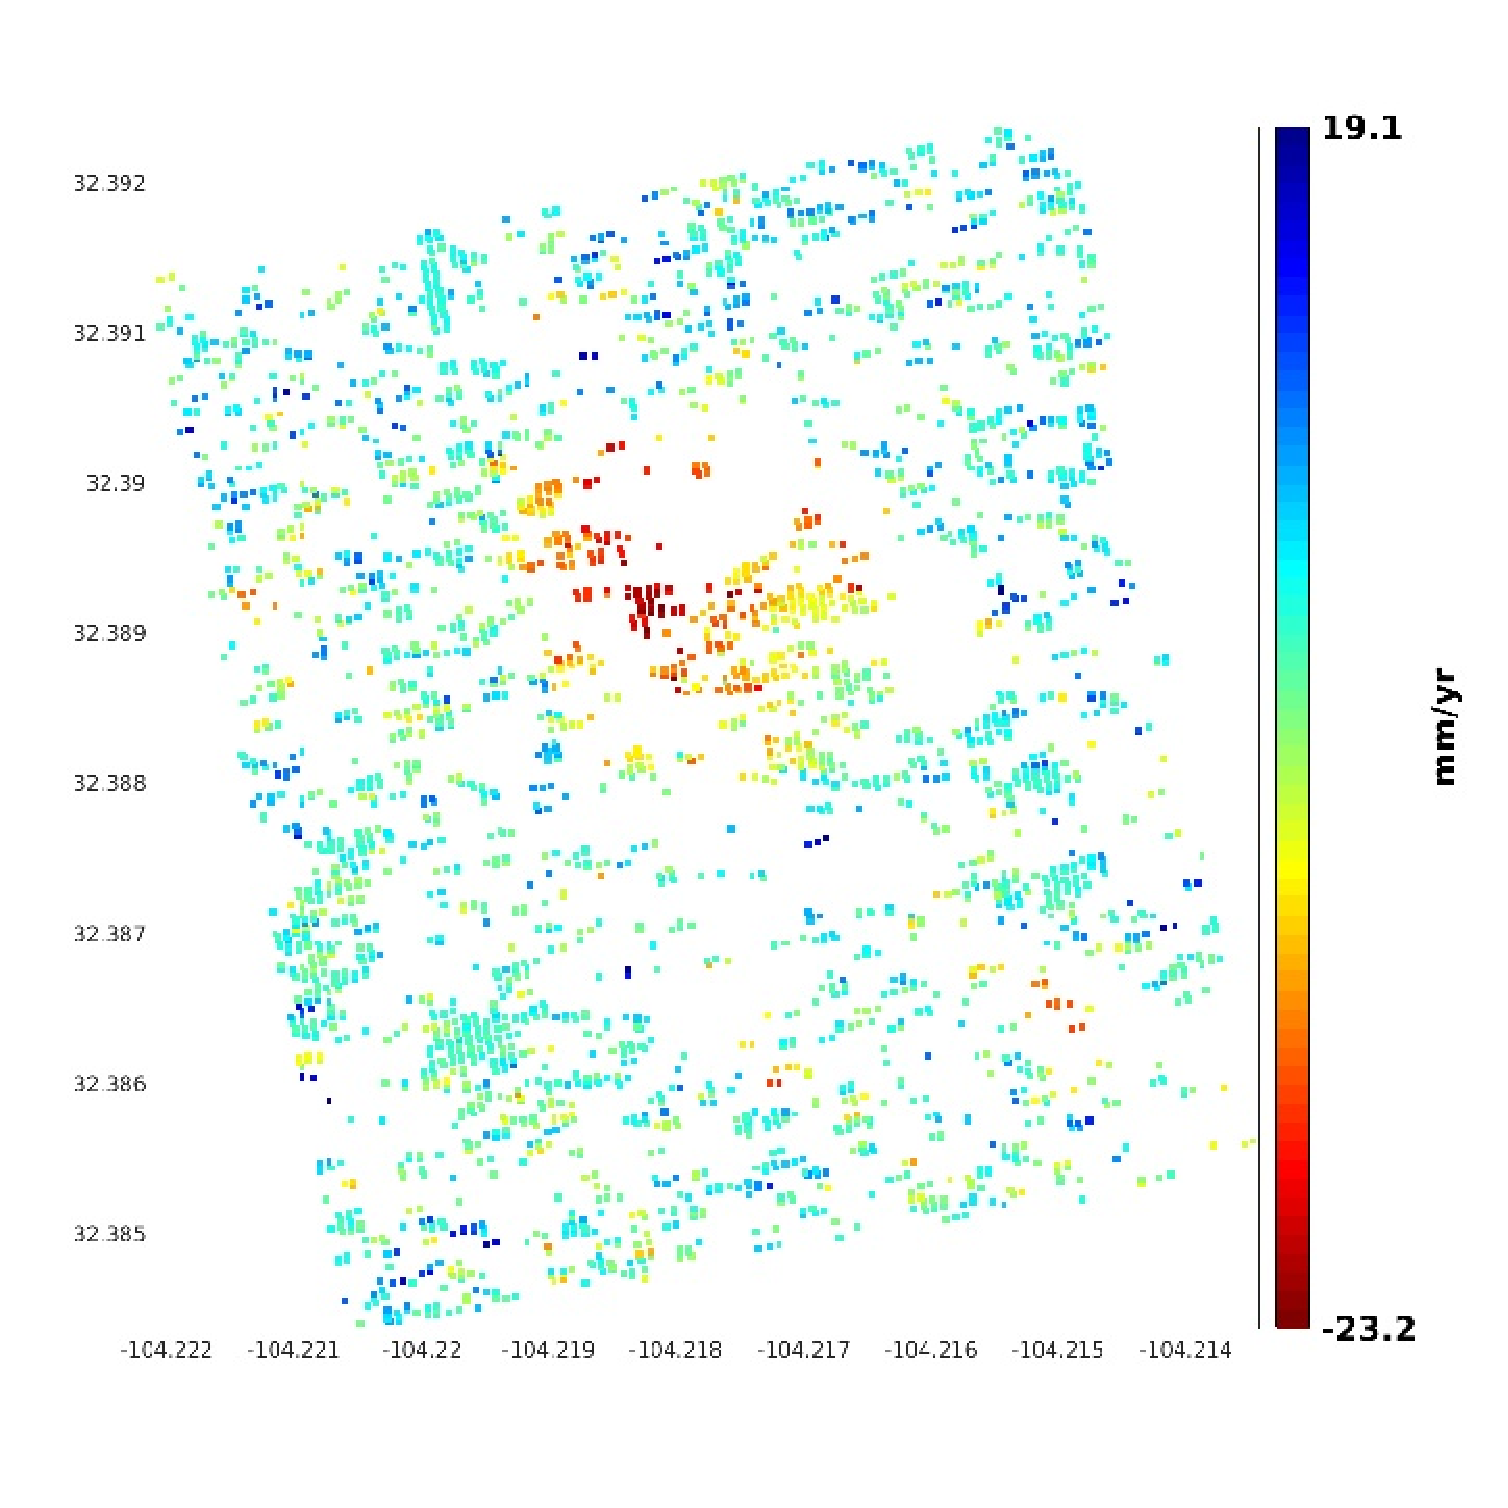
\includegraphics[width=1.0\textwidth]{sbasv.eps}
    \caption{研究区域平均沉降速率图}
    \label{fig:sbasv}
\end{figure}
\begin{figure}[htb]
    \centering
    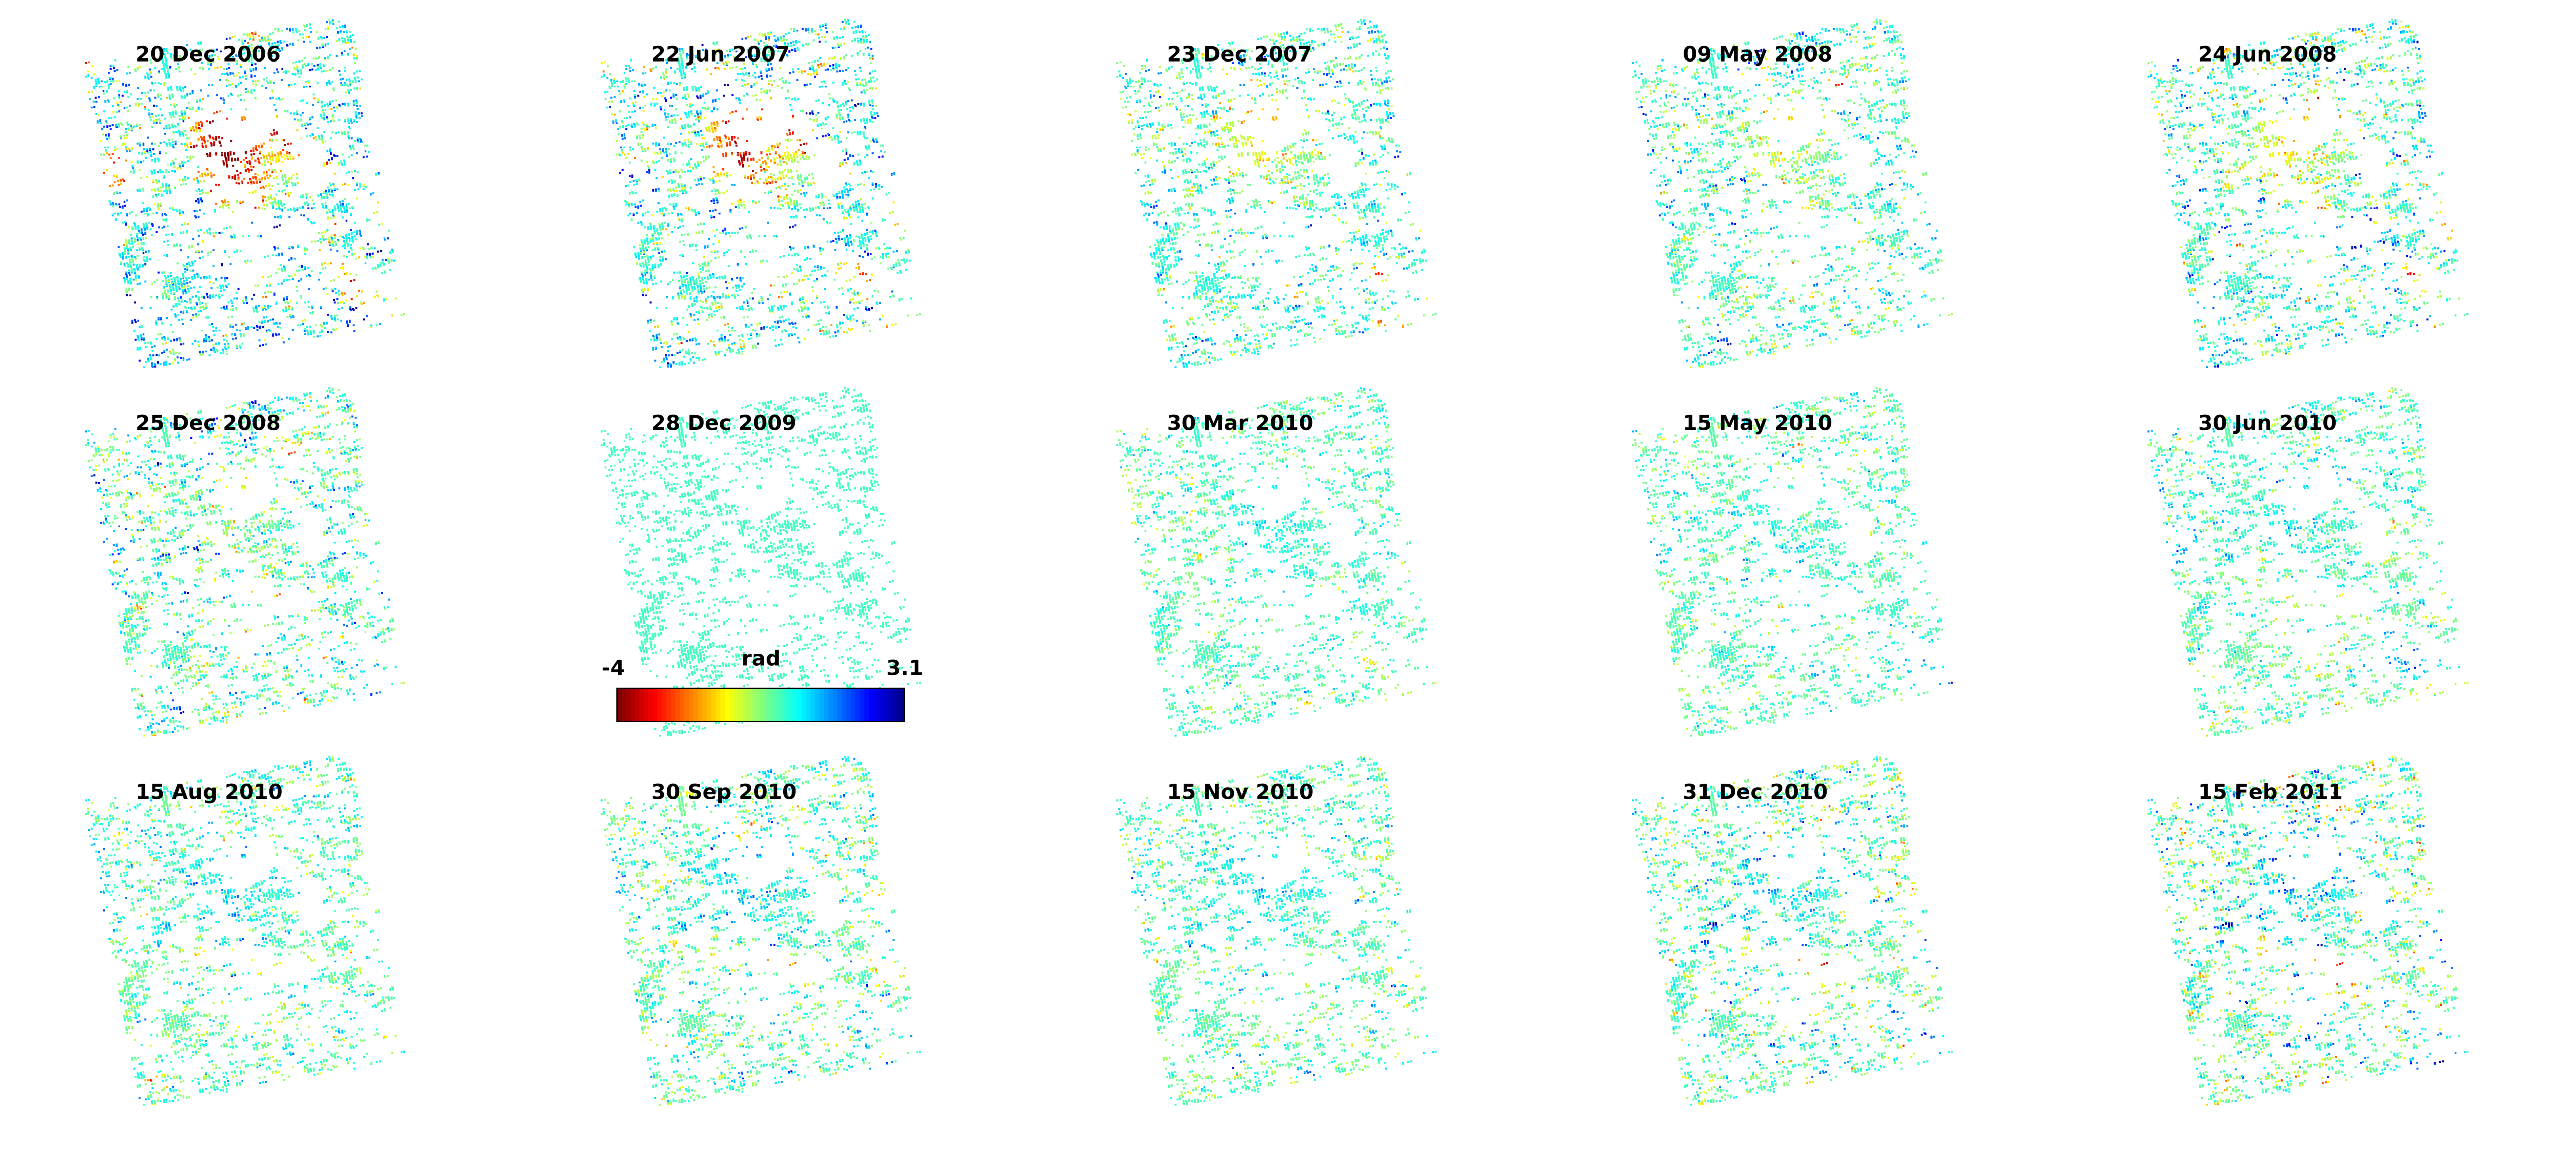
\includegraphics[width=1.0\textwidth]{sbasu.pdf}
    \caption{研究区域相对于主影像形变图}
    \label{fig:sbasu}
\end{figure}

\section{形变结果的初步分析}
从图\ref{fig:sbasv}和图\ref{fig:sbasu}中可以明显地看出中部地区有明显的沉降。
变形最明显的区域的形变可以达到平均23.2mm/year的速度,
累计最大形变可达81mm。
从形变的结果来看,此变形比较类似于点源引起的变形,下一步使用点源做一个模型。
同时,右下角部分有一定的形变,但由于在该部位所选取的PS点较少的缘故,该区域的形变很难建模。
